\chapter{Der kleine Kapiteltest}
	\blindtext

\section{Unterkapitel mit Blindtext und Bild}
	\blindtext
	
	Tabellen die zu lang sind um sie auf einer \emph{normalen} Seite darzustellen können mithilfe des \emph{lscape} Paketes um \SI{90}{\celsius} auf einer separaten Seite angezeigt werden. Dabei wird der Inhalt gedreht, die Kopf- und Fußzeile bleiben erhalten. Hierfür muss die Tabelle von einer \emph{landscape} Umgebung umschlossen werden. Ein Beispiel hierfür ist Tabelle~\ref{tbl:transparenteBoeden}.\\
	Weiterhin wurde die \emph{tabular} Umgebung um drei weitere mögliche Spaltenbezeichnungen erweitert. Die Bezeichnungen \emph{L}, \emph{M} und \emph{R} werden durch eine Option in ihrer Breite festgelegt (vgl. Tab~\ref{tbl:transparenteBoeden}). Dabei ist eigenverantwortlich darauf zu achten, dass die Tabelle nicht zu breit wird.\\
	Alternativ kann auch die Umgebung \emph{tabularx} verwendet werden, bei der die Gesamtbreite der Tabelle festgelegt wird und eine (oder mehrere) Spalte(n) als in der breite flexibel mit einem \emph{X} bezeichnet (vgl. Tab.~\ref{tbl:tabularx}).
	
	\begin{landscape}		
		\begin{table}
			\captionabove{Zusammenstellung bindiger und nicht-bindiger Bodenimitate, modifiziert nach \textcite{alireza_hassanzadegan_thermomechanical_2012}}
			\label{tbl:transparenteBoeden}
			\centering
			\begin{tabular}{L{4.0cm}C{3cm}C{3cm}C{3cm}C{3cm}C{3cm}}
				\toprule[1.5pt]
				\textbf{Eigenschaft} & \multicolumn{3}{c}{\textbf{Bindige Bodenimitate}} & \multicolumn{2}{c}{\textbf{Nicht-bindige Bodenimitate}}\\ 
				
				\midrule\midrule
				\textbf{Bezeichnung\newline(deutsch)} & amorphes \newline Siliziumdioxid, Kieselsäure & Hydro-Gel & Laponite RD® & Siliziumdioxid-Gel, Kieselgel & Quarzglas \\
				
				\midrule 
				\textbf{Bezeichnung\newline(englisch)} & amorphous silica, Silica powders & Aquabeads & Laponite RD® & Silica gels & Fused quartz, fused silica \\
				
				\midrule 
				\textbf{Brechungsindex}\newline$[-]$ & $1,442$ & $1,333$ & $1,336$ & $1,442$ & $1,458$ \\
				
				\midrule 
				\textbf{Porenfluid} & Mineralöle, Paraffinölen, Kalziumbromidlösung & Wasser & Wasser & Mineralöle, Paraffinöle, Kalziumbromidlösung & Mineralöle, STSI, Saccharoselösung \\
				
				\midrule
				\textbf{Sättigungswichte}\newline$[\SI{}{\kilo\newton\per\meter\cubed}]$ & 9,4 -- 16 & 10 & 10 & 11 -- 14 &  13,4 -- 16,4 \\
				
				\midrule
				\textbf{Reibungswinkel}\newline$[\SI{}{\degree}]$      & 19 -- 36* & -- & -- & 29 -- 42* & 44 -- 59* \\
				
				\midrule
				\textbf{Kohäsion} $[\SI{}{\kilo\newton\per\meter\squared}]$ & 20 -- 44* & 0,005 -- 0,012** & 0,3 -- 0,42** & -- & -- \\
				
				\midrule
				\textbf{Durchlässigkeit $[\SI{}{\meter\per\second}]$} & $2,3\cdot10^{-9}$ – $2,5\cdot10^{-7}$ & $6,0\cdot10^{-10}$ – $7,0\cdot10^{-4}$ & $5,0\cdot10^{-11}$ – $1,6\cdot10^{-8}$ & $1,5\cdot10^{-6}$ – $7,0\cdot10^{-5}$ & $1,3\cdot10^{-7}$ – $2,1\cdot10^{-7}$ \\
				
				\midrule
				\textbf{Ersatzmaterial} & Ton & sehr weicher Ton & sehr weicher Ton & Fein- bis Grobsand & Feinsand bis Mittelkies \\
				
				\midrule[1.5pt]
				\multicolumn{6}{l}{\footnotesize *drainiert \quad **undrainiert}\\
				%\bottomrule [1.5pt]
			\end{tabular}
		\end{table}
	\end{landscape}
	
	\begin{figure}[h]
		\centering
		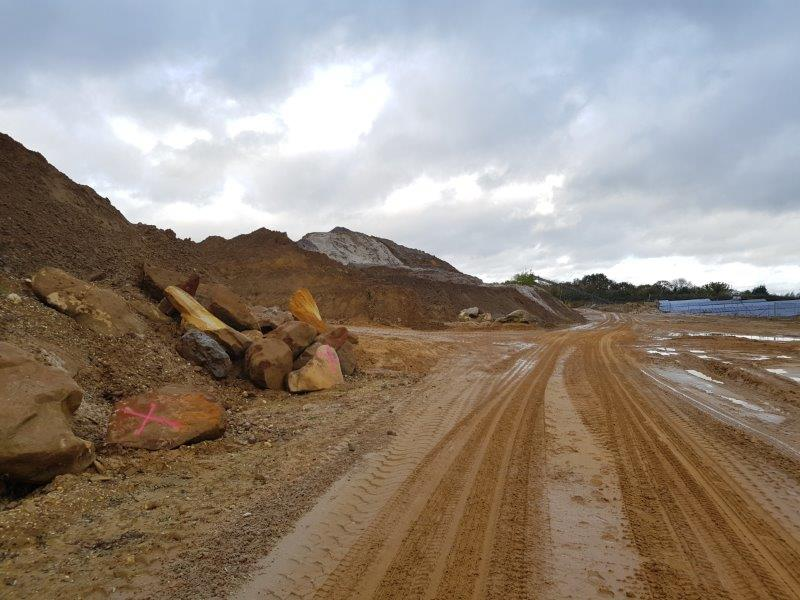
\includegraphics[width=0.9\linewidth]{20191112_111105.jpg}  % picked from the defined standard folder 'figures/'
		\caption{Nievelsteiner Steinbruch}
		\label{fig:20191112111105}
	\end{figure}


\section{Unterkapitel mit Beispielen}
	Griechische Buchstaben können direkt eingetippt werden. So kann α anstatt \$\textbackslash alpha\$ (o.~ä.) im Fließtext verwendet werden.
	
	Es folgt ein Beispiel für die Verwendung von Abkürzungen:
	\begin{itemize}
		\item erstes auftreten der Abkürzung: \ac{ufo}
		\item zweites auftreten der Abkürzung: \ac{ufo}
		\item volle Ausgabe der Abkürzung: \acf{ufo}
		\item Langfassung der Abkürzung: \acl{ufo}
		\item kurzfassung der Abkürzung: \acs{ufo}
	\end{itemize}
	
	Noch ein weiteres Beispiel für die Verwendung von Abkürzungen:
	\begin{itemize}
		\item erstes auftreten der Abkürzung: \ac{3ax}
		\item zweites auftreten der Abkürzung: \ac{3ax}
	\end{itemize}
	
	Im folgenden wird gezeigt, dass die deutsche Notation für die Darstellung von Zahlen verwendet wird. Dabei ist das ``,'' das Dezimaltrennzeichen und ein ``.'' ein Tausendertrennzeichen, wobei der Punkt durch ein halbes Leerzeichen ersetzt wird.\\
	\begin{math}
		1 + 2,3\cdot 4.500 - 8.000,500654 = 54,3 \alpha
	\end{math}
	
	Hier wird die Nummerierung von Formeln gezeigt:
	\begin{equation}
		a=b
	\end{equation}
	
	\begin{table}
		\captionabove{Versuchsplanung Übersicht}
		\label{tbl:tabularx}
		\centering
		\begin{tabularx}{8cm}{lrX} 
			\toprule
			Fach & Dauer & Einkommen (€)\\ 
			\midrule 
			Bauing & 10 & $45.000$ \\
			WirtIng & 6 & $65.000$ \\
			AngewGeoW & 8 & $35.000$\\ 
			\bottomrule
		\end{tabularx}
	\end{table}


\subsection{Unterunterkapitel 1}
	Hier werden nun ein paar Zitationen vorgestellt. Es gibt solche im Text von \textcite{alam_effects_2014} und jene die am Ende eines Abschnitts stehen. \parencites{bailey_technology_2018}{alam_effects_2014}{dassault_systemes_abaqus_2017}{dassault_systemes_abaqus_2019}
	\\
	\cite{richardson_permeability_1987}
	Außerdem können wir durch das Paket \emph{siunitx} sehr einfach Zahlen mit Einheiten, bspw.	\SI{35.8}{\kilo\newton\per\square\meter} oder eine Bandbreite \SIrange{1e-9}{10e-9}{\meter\per\second} angegeben. Hierbei wird immer ein geschütztes Leerzeichen zwischen die Zahl und die Einheit gesetzt.
	
	\blindtext \parencite{alireza_hassanzadegan_thermomechanical_2012}